\documentclass[a4paper]{article}

\usepackage{pdp}

%------------------------------------------------------------------------------
%	REPORT INFORMATION
%------------------------------------------------------------------------------

\title{Carcassonne -- Python}
\subtitle{Rapport préliminaire}
\author{Loïc THIN, Tony HUANG, Clément SIMON, Anthony BEAUVIEUX, Maxence SALIN}
\date{}

%------------------------------------------------------------------------------

\begin{document}

%------------------------------------------------------------------------------
%	TITLE PAGE
%------------------------------------------------------------------------------

\maketitle
\thispagestyle{empty}

%------------------------------------------------------------------------------
%	MAIN MATTER
%------------------------------------------------------------------------------

\section{Présentation du jeu}

\subsection{Contexte}

\textbf{Carcassonne} est un jeu de stratégie et de placement de tuiles créé par \textsf{Klaus-Jürgen Wrede} en 2000, conçu pour 2 à 5 joueurs, et pouvant accueillir jusqu'à 6 joueurs grâce à l'extension \textit{The River}. Il s'agit d'un jeu stochastique à information parfaite,
 c'est-à-dire un jeu où le hasard intervient dans le tirage des tuiles mais où l’ensemble des éléments présents sur le plateau est visible de tous les joueurs.

La version considérée ici utilise les 72 tuiles du jeu de base, auxquelles s'ajoutent les 12 tuiles de l'extension \textit{The River}. Chaque joueur dispose de 8 pions de sa couleur pour marquer des points au cours de la partie.

Le but du jeu est que les joueurs construisent progressivement le plateau, à tour de rôle, en posant des tuiles de manière cohérente et en plaçant stratégiquement leurs pions pour accumuler des points. Le vainqueur est le joueur qui totalise le plus de points à la fin de la partie.


\subsection{Règles}

Les règles de \textbf{Carcassonne} utilisées sont celles de la version 2012\cite{rulescarcassonne}.

\subsubsection{Spécificités}
\begin{description}[style=nextline]
  \item[Tuile] Chaque tuile possède quatre côtés ainsi qu’un centre.
  Chaque côté correspond à un type de terrain parmi \textit{Road}, \textit{City} ou \textit{Field}.
  Le centre peut représenter une \textit{City}, un \textit{Field}, une \textit{Banner} ou un \textit{Monastery}.
  \begin{figure}[H]
    \centering
    
  \begin{minipage}{0.35\textwidth}
    \centering
    \frame{
\includegraphics[width=0.25\textwidth]{images/carcassonne_example_tile_CFRR.png}}
    \caption{Exemple d'une tuile avec une \textit{City}, une \textit{Road} et un \textit{Field}}\label{fig:exemple_tuile_1}
  \end{minipage}
  \hspace{0.5cm}
 \begin{minipage}{0.35\textwidth}
    \centering
    \frame{
\includegraphics[width=0.25\textwidth]{images/carcassonne_example_tile_banner.png}}
    \caption{Exemple d'une tuile où une \textit{City} possède une \textit{Banner}}\label{fig:exemple_tuile_2}
  \end{minipage}
  
  \end{figure}

  \item[Pion] Lorsqu’un pion est placé sur une tuile, il prend un rôle en fonction du type de terrain occupé :
  \textit{Knight} sur une \textit{City}, \textit{Farmer} sur un \textit{Field}, \textit{Thief} sur une \textit{Road}
  et \textit{Monk} sur un \textit{Monastery}.
\end{description}


\subsubsection{Début de partie}
\begin{itemize}
  \item[$\bullet$] Nombre de joueurs : de 2 à 6, chacun associé à une couleur.
  \item[$\bullet$] Pions : chaque joueur dispose de 8 pions de sa couleur.
  \item[$\bullet$] Tuile initiale : une tuile avec une \textit{City} en haut, une \textit{Road} qui traverse de gauche à droite et une \textit{Field} en bas (notée CRFR) est placée au centre du plateau.
  \begin{figure}[H]
    \centering
    \frame{
\includegraphics[width=0.1\textwidth]{images/carcassonne_starting_tile.png}}
    \caption{Tuile de départ}\label{fig:tuile_de_départ}
  \end{figure}
  \item[$\bullet$] Pioche principale : 71 tuiles du jeu de base, placées face cachée.
\end{itemize}

\subsubsection{Règles d'un tour de jeu}

Les joueurs jouent à tour de rôle selon un ordre prédéfini (généralement dans le sens horaire, en commençant par le joueur le plus jeune).  
À son tour, un joueur effectue les actions suivantes dans l’ordre indiqué :

\begin{enumerate}
  \item \textbf{Piocher une tuile}  
  Le joueur pioche une tuile dans la pioche actuellement active. Cette tuile est visible par l’ensemble des joueurs.

  \item \textbf{Placer la tuile}  
  La tuile piochée doit être placée sur le plateau en respectant les règles suivantes :
  \begin{itemize}
    \item[-] La tuile doit être adjacente à au moins une autre tuile déjà posée.
    \item[-] Les côtés en contact doivent être de même type de terrain.
  \end{itemize}

  \item \textbf{Placer un pion (optionnel)}  
  Le joueur peut placer un pion sur une partie de la tuile qu’il vient de poser (un des quatre côtés ou le centre).

  \item \textbf{Restriction de placement des pions}  
  Si une partie de terrain de la tuile posée est reliée à une partie du même type déjà occupée par un pion, aucun nouveau pion ne peut y être placé.  
  Les \textit{Road} et \textit{City} agissent comme des séparateurs entre les terrains.

  \item \textbf{Résolution des terrains complétés}  
  Si la pose de la tuile complète un ou plusieurs terrains, ceux-ci sont résolus immédiatement :
  \begin{description}[style=nextline]
    \item[Road]
    Une route est complète lorsque ses deux extrémités atteignent une intersection ou une fin de route.
    Le joueur possédant le plus de pions (\textit{Thief}) sur cette route gagne un nombre de points égal au nombre de tuiles composant la route.
    En cas d’égalité, tous les joueurs concernés marquent ces points.

    \item[City]
    Une ville est complète lorsqu’elle est entièrement fermée.
    Le joueur possédant le plus de pions (\textit{Knight}) gagne 2 points par tuile composant la ville, ainsi que 2 points par \textit{Banner}.
    En cas d’égalité, les points sont attribués à tous les joueurs concernés.

    \item[Monastery]
    Un monastère est complet lorsque les 8 cases entourant sa tuile sont occupées.
    Le joueur possédant le pion dans le \textit{Monastery} (\textit{Monk}) gagne alors 9 points.

    \item[Field]
    Les champs ne sont résolus qu’à la fin de la partie.
    Un pion dans un \textit{Field} (\textit{Farmer}) reste donc en jeu jusqu’à la fin.
  \end{description}

  \item \textbf{Retour des pions}  
  Tous les pions associés à des \textit{City}, \textit{Road} ou \textit{Monastery} complétés durant ce tour sont retirés du plateau et rendus à leurs propriétaires.
\end{enumerate}

\begin{figure}[H]
    \centering
    \frame{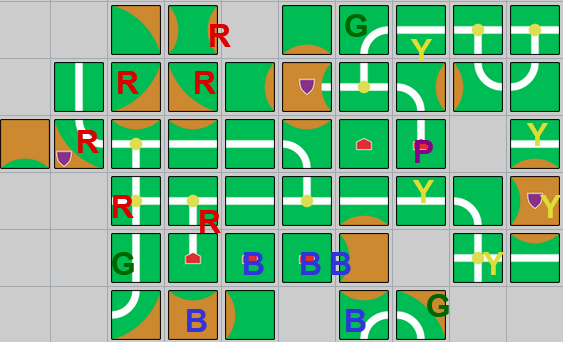
\includegraphics[width=0.8\textwidth]{images/carcassonne_exemple_partie.png}}
    \caption{Exemple d'un plateau d'une partie en cours (les lettres correspondent aux pions de chaque joueurs)}\label{fig:exemple_partie}
  \end{figure}


\subsubsection{Fin de partie}

La partie prend fin lorsqu’il n’y a plus de tuiles dans la pioche principale.
Les joueurs ajoutent alors à leur score les points correspondant aux terrains non complétés,
selon les règles suivantes :

\begin{description}[style=nextline]
  \item[Road]
  Une route incomplète rapporte 1 point par tuile la composant au joueur possédant le plus de pions (\textit{Thief}) sur cette route.
  En cas d’égalité, tous les joueurs concernés marquent ces points.

  \item[City]
  Une ville incomplète rapporte 1 point par tuile la composant ainsi que 1 point par \textit{Banner} présent,
  pour le joueur possédant le plus de pions (\textit{Knight}).
  En cas d’égalité, les points sont attribués à tous les joueurs concernés.

  \item[Monastery]
  Un monastère incomplet rapporte 1 point par tuile adjacente, y compris la tuile du monastère,
  pour un total compris entre 2 et 8 points.

  \item[Field]
  Chaque \textit{Farm} (ensemble de \textit{Field} connectés ; un \textit{Field} isolé constitue une \textit{Farm})
  est attribuée au joueur possédant le plus de pions (\textit{Farmer}).
  Ce joueur marque 3 points par \textit{City} complète adjacente à la \textit{Farm}.
  En cas d’égalité, les points sont attribués à tous les joueurs concernés.
\end{description}

Le joueur ayant obtenu le plus grand nombre de points à l’issue du décompte final remporte la partie.

\subsubsection{Extension : \textit{The River}}

L’extension \textit{The River} introduit 12 tuiles supplémentaires et modifie la phase de mise en place du jeu.
En début de partie, avant toute pose de tuile du jeu de base, les joueurs utilisent une pile de tuiles distinctes afin de construire un cours d’eau.
La tuile \textit{Spring} est placée en premier, tandis que la tuile \textit{Lake} est réservée et placée en dernière position. (A noté que la tuile \textit{Spring} et \textit{Lake} sont identiques visuellement, mais différenciées par leur nom.)
Les tuiles de rivière restantes sont mélangées. À tour de rôle, chaque joueur en pose une afin de former une ligne continue et sinueuse.
Chaque tuile doit être disposée de manière à assurer la correspondance des types de terrain sur les côtés adjacents.
Le cours d’eau se termine par la tuile \textit{Lake} qui remplace la tuile de départ habituelle.
Une fois la rivière complétée, la partie se poursuit selon les règles standard de \textit{Carcassonne}, sur un terrain initialement structuré.

\begin{figure}[H]
    \centering
    \frame{
\includegraphics[width=0.1\textwidth]{images/carcassonne_example_tile_theriver.png}}
    \caption{Tuile \textit{Spring} et tuile \textit{Lake} de l'extension \textit{The River}}\label{fig:tuile_The_River}
  \end{figure}


\subsection{Complexité}

\textbf{Carcassonne} est un jeu aux règles simples, mais qui offre une grande richesse stratégique, les choix des joueurs se complexifiant à mesure que le plateau s’étend. 
Ainsi, sa complexité est comparable à celle de jeux classiques comme les échecs ou le go.

\begin{figure}[H]
    \centering
    \frame{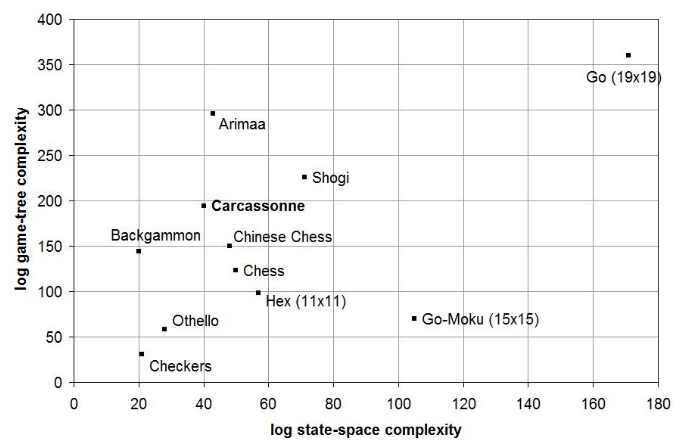
\includegraphics[width=0.8\textwidth]{images/carcassonne_complexite.png}}
    \caption{Comparaison de la complexité de Carcassonne avec d'autres jeux \cite{heydencarcassonne}}
    \label{fig:complexite_carcassonne}
\end{figure}

La complexité combinatoire du jeu est particulièrement élevée en raison du grand nombre de tuiles et des multiples façons dont elles peuvent être placées sur le plateau, ainsi que des stratégies variées que les joueurs peuvent adopter selon la configuration des tuiles et la position des pions. 
La complexité de l’arbre de jeu est estimée à environ $10^{194}$ \cite{heydencarcassonne}, ce qui rend toute résolution complète du jeu par des méthodes de recherche exhaustive irréaliste. 
Par conséquent, la création d’une intelligence artificielle capable de jouer parfaitement à \textbf{Carcassonne} devient impossible.


\section{Algorithmes et structures de données}

\section{Architecture}

\section{Spécifications étendues}

\pgfplotstabletypeset[
  col sep=semicolon,
  string type,
  every head row/.style={before row=\toprule, after row=\midrule},
  every last row/.style={after row=\bottomrule}
]{agenda_besoin_PDP.csv}
%------------------------------------------------------------------------------
%	BIBLIOGRAPHY
%------------------------------------------------------------------------------
\newpage

\nocite{*}
\bibliographystyle{plain}
\bibliography{bibliography}

\end{document}
